Use the finite element method to solve the differential equation
\[ -(u'(x) \kappa(x))' = 2x, \qquad 0<x<1\]
for $\kappa(x) = 1+x^2$, subject to homogeneous Dirichlet boundary conditions,
\[ u(0) = u(1) = 0,\]
with the approximation space $V_N$ given by the piecewise linear
\emph{hat functions} that featured on earlier problem sets:
For $n\ge 1$,  $h = 1/(N+1)$,  and $x_k = kh$ for $k = 0, \ldots, N+1$,
we have 
\[ \phi_k(x) = \left\{ \begin{array}{ll}
           (x-x_{k-1})/h, & x\in [x_{k-1}, x_k);\\
           (x_{k+1}-x)/h, & x\in [x_k, x_{k+1});\\
            0,             & \mbox{otherwise}.
          \end{array}\right. \]

\begin{enumerate}
\item Write MATLAB code that constructs the stiffness matrix $\BK$ for a given value of $N$,
      with $\kappa(x) = 1+x^2$.

      [You may edit the \verb|fem_demo1.m| code from the class website.
       You should compute all necessary integrals (by hand or using a symbolic package)
       so as to obtain clean formulas that depend on $h$ and the index of the hat functions
       involved (e.g.,$a(\phi_j, \phi_j)$ can depend on $j$).]

\vspace*{1em}
\item Write MATLAB code that constructs the load vector $\Bf$ for a given value of $N$, 
       with $f(x) = 2x$.  
         
\vspace*{1em}
\item For $N = 7$ and $N=15$, produce plots comparing your solution $u_N$
      to the true solution 
               \[ u(x) = (4/\pi) \tan^{-1}(x) - x. \]
      (Note that you can compute $\tan^{-1}(x)$ as {\tt atan(x)} in MATLAB.)
      
\vspace*{1em}
\item Produce a \verb|loglog| plot showing how the error 
      \[ \max_{x\in [0,1]} |u_N(x) - u(x)| \]
      decreases as $N$ increases.
      (For example, take $N=8,16,32,64,128, 256, 512$.)  
      On the same plot, show $N^{-2}$ for the same values of $N$.
      If your code from parts~(a) and~(b) is working, your error curve
      should have the same slope as the $N^{-2}$ curve.
      (Consult the \verb|fem_demo1.m| code on the website
      for a demonstration of the style of plot we intend for part~(d);
      edit this code as you like.)
\end{enumerate}

%%%%%%%%%%%%%%%%%%%%%%%%%%%%%%%%%%%%%%%%%%%%%%%%%%%%%%%%%%%%%%%%%%%%%%%%%%%%%%%%

\ifthenelse{\boolean{showsols}}{\newpage\begin{solution}
\begin{enumerate}
\item First we compute the energy inner product of the basis functions.  Note that
\[ {d\phi_k\over dx}(x) = \left\{ \begin{array}{ll}
           1/h, & x\in [x_{k-1}, x_k);\\
           -1/h, & x\in [x_k, x_{k+1});\\
            0,             & \mbox{otherwise}.
          \end{array}\right. \]
Thus we have
\begin{eqnarray*}
a(\phi_j,\phi_j) &=& \int_0^1 (1+x^2) \Big({d\phi_j\over dx}(x)\Big)^2\,dx \\[0.5em]
                 &=& \int_{x_{j-1}}^{x_j} (1+x^2) \Big({1\over h}\Big)^2\,dx 
                     + \int_{x_j}^{x_{j+1}} (1+x^2) \Big(-{1\over h}\Big)^2\,dx \\[0.5em]
                 &=& {1\over h^2} \int_{x_{j-1}}^{x_{j+1}} (1+x^2) \,dx 
                 \ =\  {1\over h^2} \Big[ x + {x^3\over 3}\Big]_{x_{j-1}}^{x_{j+1}} 
                 \ =\ {2\over h} + {2h \over 3} + 2hj^2,
\end{eqnarray*}
\begin{eqnarray*}
a(\phi_j,\phi_{j+1}) &=& \int_0^1 (1+x^2) \Big({d\phi_j\over dx}(x)\Big)
                                          \Big({d\phi_{j+1}\over dx}(x)\Big)\,dx \\[0.5em]
                 &=& \int_{x_{j}}^{x_{j+1}} (1+x^2) \Big(-{1\over h}\Big)({1\over h}\Big)\,dx  \\[0.5em]
                 &=& -{1\over h^2} \int_{x_{j}}^{x_{j+1}} (1+x^2) \,dx 
                 \ =\ -{1\over h^2} \Big[ x + {x^3\over 3}\Big]_{x_j}^{x_{j+1}} 
                 \ =\ -{1\over h} - h\Big(j^2 + j + {1\over 3}\Big),
\end{eqnarray*}
and  for $|j-k|>1$,
\[ a(\phi_j, \phi_k) = 0\]
since $\big(d\phi_j(x)/dx\big) \big(d\phi_k(x)/dx \big) = 0$ for all $x\in[0,1]$
(except at the nodes $x_\ell$, where strictly speaking these derivatives are not 
defined---but these single isolated points do not add anything to the integral).
The stiffness matrix is given by
\[ \textbf{K} = \left[\begin{array}{ccc} a(\phi_1,\phi_1) & \cdots & a(\phi_1,\phi_n) \\
                           \vdots & \ddots & \vdots \\
                          a(\phi_n,\phi_1) & \cdots & a(\phi_n, \phi_n)\end{array}\right].\]
\item
Next we compute the entries of the load vector:
\begin{eqnarray*}
(f,\phi_j) &=& \int_0^1 f(x) \phi_j(x)\,dx \\[0.5em]
           &=& \int_{x_{j-1}}^{x_{j}} (2x)\Big( {x-x_{j-1} \over h}\Big)\, dx 
              +\int_{x_{j}}^{x_{j+1}}  (2x)\Big( {x_{j+1}-x \over h}\Big)\, dx  \\[0.5em]
           &=& {1\over h}\Big[ {2x^3\over 3}  - x^2 x_{j-1}\Big]_{x_{j-1}}^{x_j}
              +{1\over h}\Big[ x^2 x_{j+1} - {2x^3 \over 3} \Big]_{x_{j}}^{x_{j+1}} \\[0.5em]
           &=&  2h^2 j.
\end{eqnarray*} 
The load vector is given by
\[ \textbf{f} = \left(\begin{array}{cc} (f,\phi_1) \cr \vdots \cr (f,\phi_n)\end{array}\right).\] 
The MATLAB code at the end of this problem shows generates these matrices
and produces plots similar to those shown in (b) and (c).

\item The following plots show the solution (and error) at $N=7$ (left) and $N=15$ (right).
\begin{center} 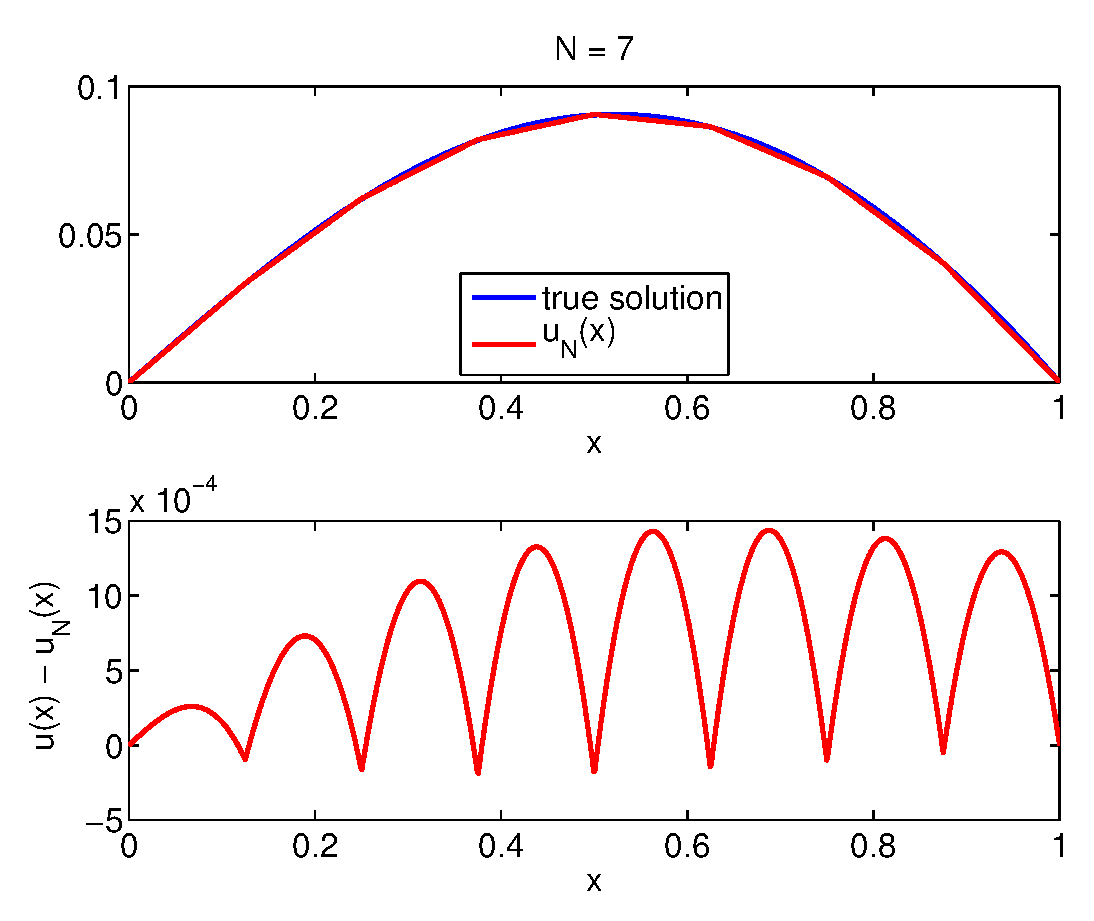
\includegraphics[scale=0.4]{fema7} \quad
               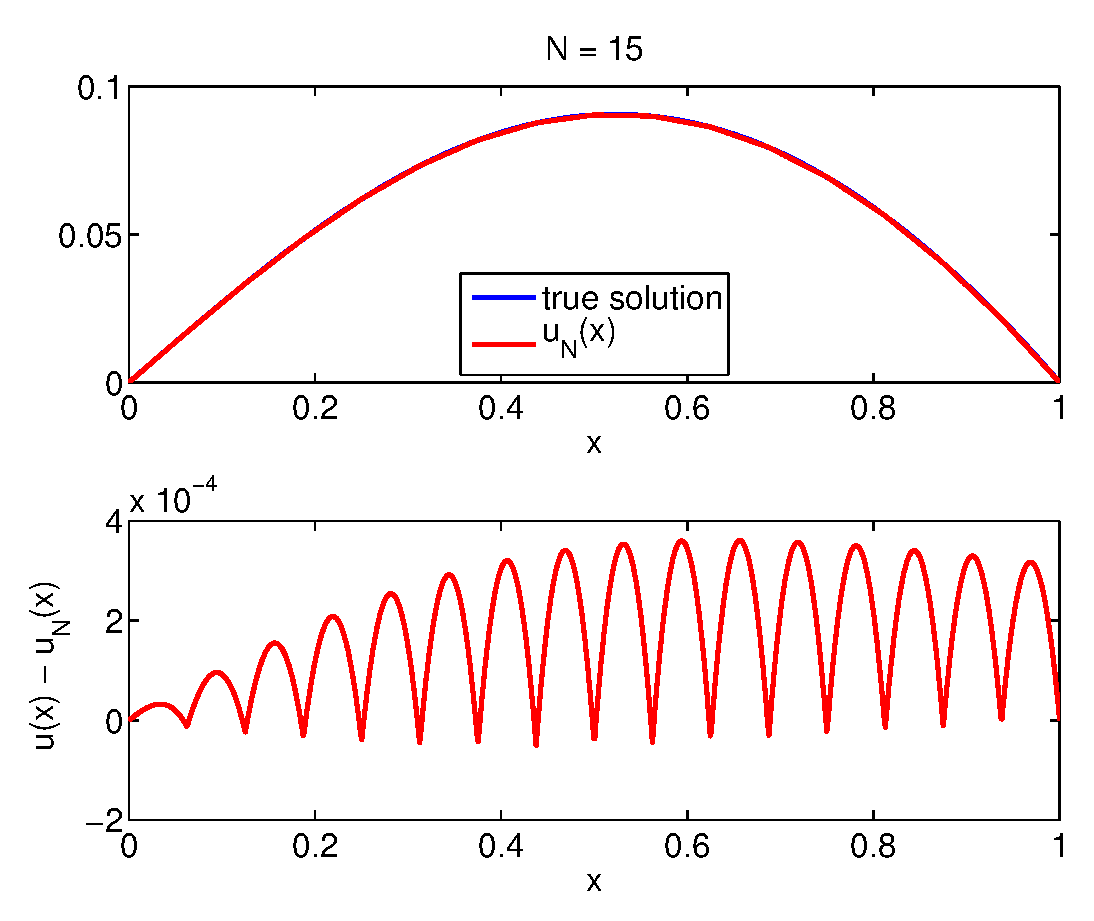
\includegraphics[scale=0.4]{fema15} 
\end{center}

\item
The following plot shows the decay of the error as a function of $N$.
Notice that the error decays like $1/N^2$.
\begin{center} 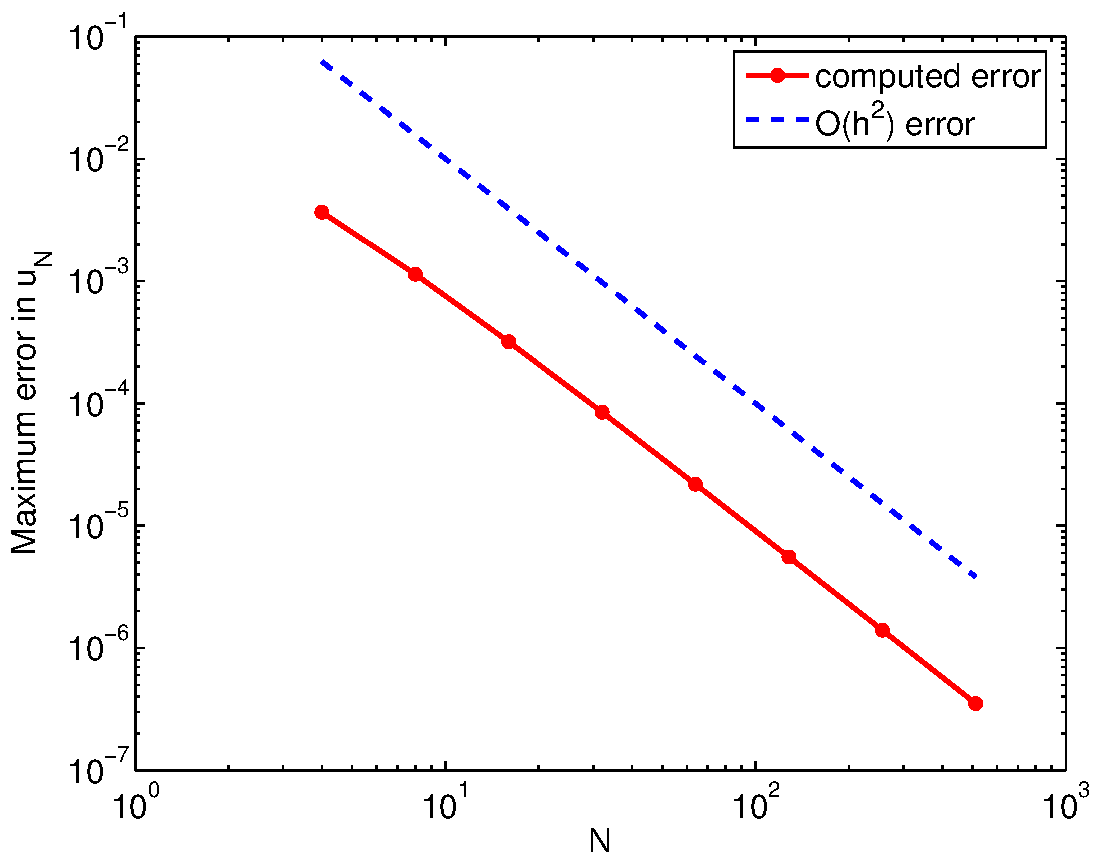
\includegraphics[scale=0.6]{femb}
\end{center}

\input fem_code
\end{enumerate}
\end{solution}}{}

